\section{Stoffwechsel}
\label{sec:stoffwechsel}
\subsection{Phototrophie}
\begin{description}
	\item[ATP-Produktion]	\hfill \\
	\item[Reduktion von Kohlenstoffdioxid]	\hfill	\\
		mit \ce{NADH} und \ce{NADPH},
		welche durch die vorherige Reduktion von \ce{NAD+} bzw. \ce{NADP*} erzeugt wurden.
\end{description}
	Bei beiden Photosynthesevarianten finden
	verschiedener akzessorischer Proteine und Photosystheme verwendung.
	Dies ermöglich die Anpassung an verschiedene Lebensräume,
	und die Anpassung an die vorhanden Lichtspektren.

\subsubsection{Oxygenen Photosynthese}
	\begin{itemize}
		\item Kein zyklischer Elektronen Transport
		\item Z-Schema mit zwei Photosysteme, (II:P680;I:P700)
	\end{itemize}

\subsubsection{Anoxygene Photosynthese}
	\begin{itemize}
		\item zyklischer Elektronen Transport
		\item Ein Photosystem (P870)
		\item umgekehrter, energieverbrauchender Elektronentransport,
			wenn \ce{NAD(P)H} nötig
	\end{itemize}

\subsubsection{\ce{CO2}-Fixierung}
\begin{description}
	\item[Calvin-Zyklus] ist am weitesten verbreitet.
		Mit den Schlüsselenzymen RUBISCO und Phosphoribulose-Kinase
		erfolgt die Bindung von \ce{CO2} in Glucose
		unter Verbrauch von \ce{ATP} und \ce{NADPH}.
		Siehe Abbildung \ref{fig:calvin_detail}.

	\item[Hydroxypropionat-Weg] der Grünen-Schwefelbakterien.
		Letzlich wird in zwei Zyklen zunächst zwei Moleküle \ce{CO2}
		in Form von Bicarbonat (\ce{HCO3-}) fetgelegt.
		Das Bicarbonat wird dann unter ATP und NADPH Verbrauch zu Glyoxalat aufgebaut.

		Anschließend werden zwei Glyoxalat Moleküle zu Pyruvat umgebaut.

	\item[umgekehrter Citrat-Zyklus] ist die Umkehrung des oxidativen Citratzyklus,
		deshalb auch reduktiver Citrat-Zyklus.
		Die Reaktionen innerhalb des oxidativen Zyklus werden dabei umgekehrt
		unter Umgehung bzw. der Verwenugn spezialisierter Moleküle für die 
		drei Unumkerhbahren Schritte des oxidativen Citrat-Zyklus.

\end{description}

\subsection{Glykolyse (EMP)}
\label{sec:glykolyse}
\begin{itemize}
	\item Ausgeglichene Oxidations-Reduktions-Reaktion
	\item Endprodukt Pyruvat
	\item Ausgangspunk für Fermentation und aerobe Atmung
	\item Weiter Produkte: Reduktionsäquivalent \ce{NADH+}
	\item Verbraucht: 2 ATP
	
\end{itemize}

\begin{enumerate}
	\item Stufe: Vorbereitende Reaktion
	\item Stufe: Synthese von ATP und Pyruvat
	\item Sutfe: Bildung von Fermentationsprodukten, aerobe Atmung
\end{enumerate}

\begin{figure}[htb!]
	\leavevmode
	\begin{center}
		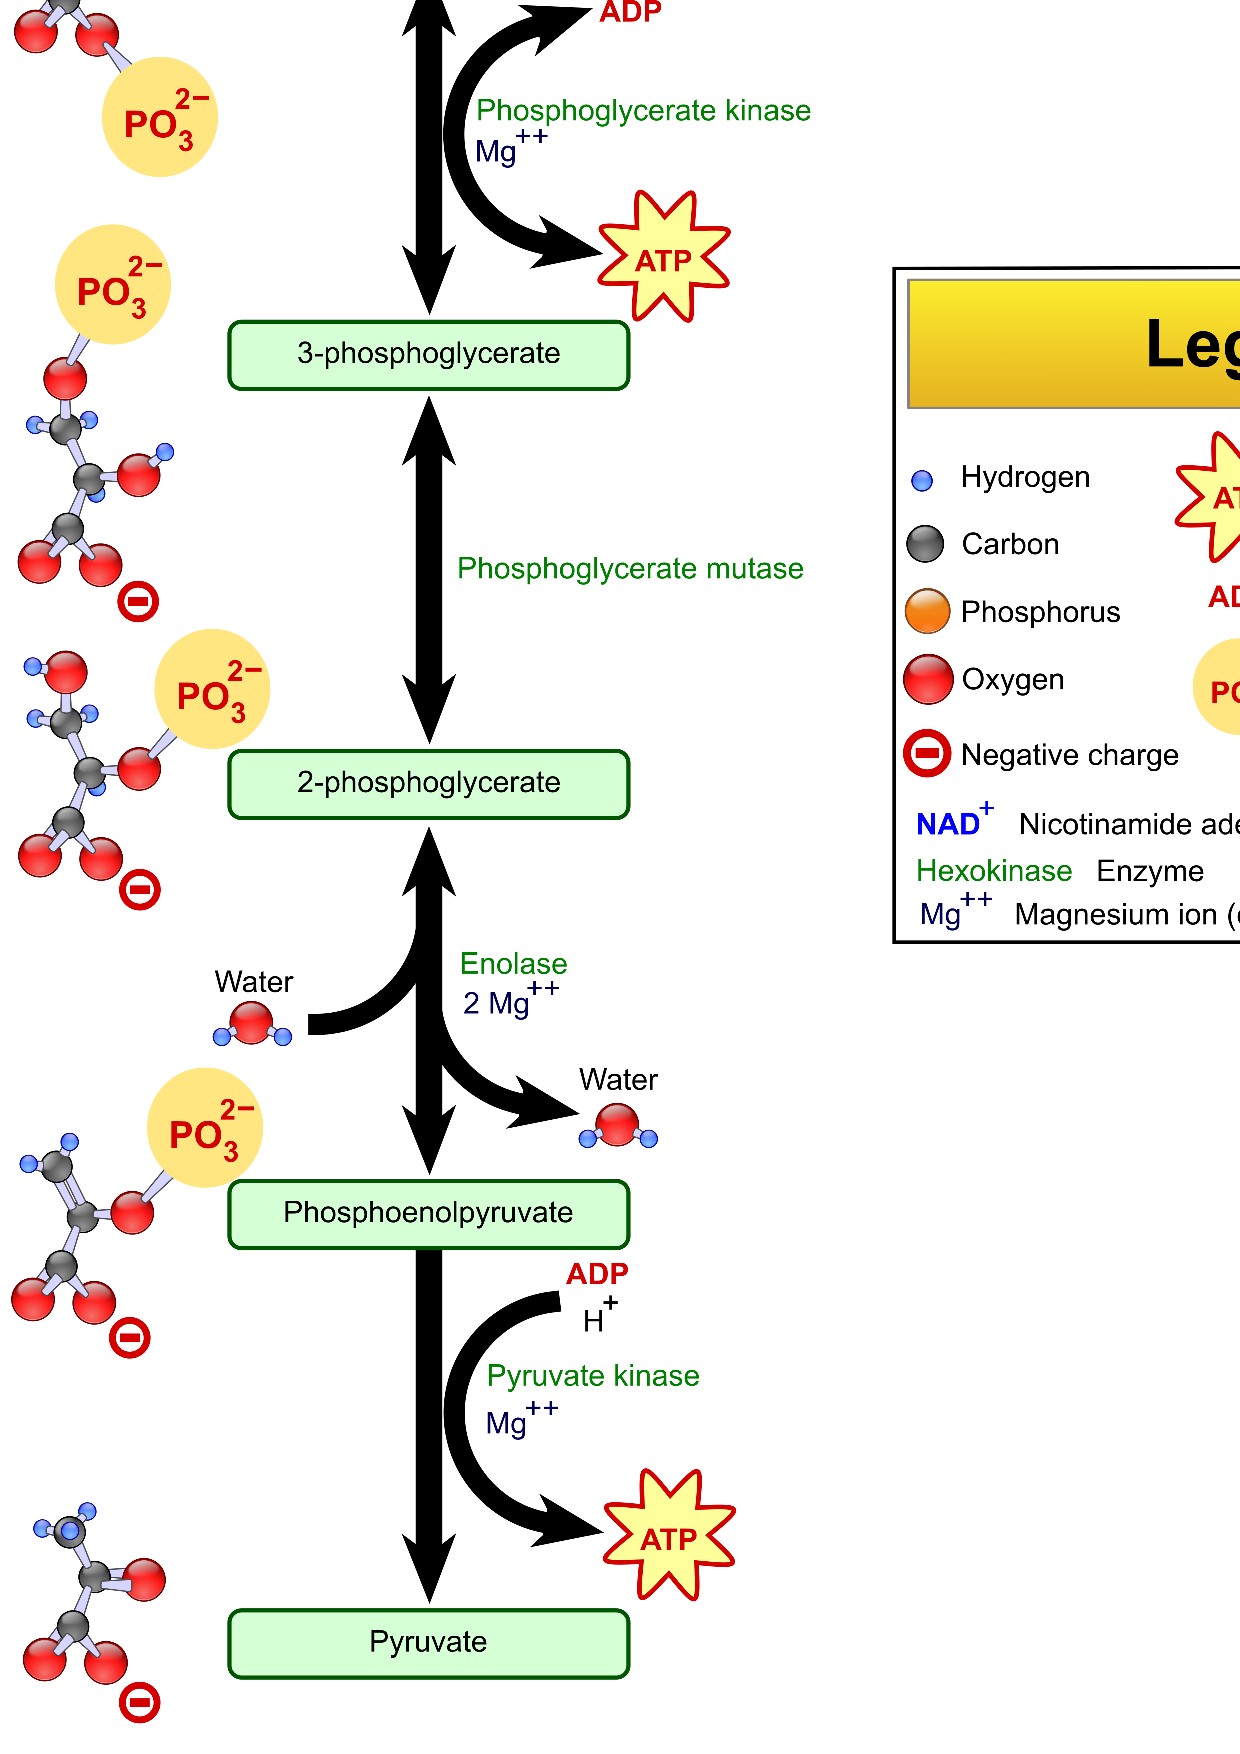
\includegraphics[scale=0.30]{./pictures/glykolysis_2k.pdf}
	\end{center}
	\caption{\slshape{Übersich über die Glykolyse.}}
	\label{fig:glykolyse}
\end{figure}

\subsection{Aerober Stoffwechsel}

\subsubsection*{Aerobe Atmung}
Die Anaerobe Atmung ist ein Stoffwechselvorgang,
zur Energieerzeung.
Durch oxidative biochemische Reaktionen wird dabei ATP erzeugt.
Sie fasst die folgenden Schritte zusammen:

\begin{description}
	\item[Gylkolyse]	\hfill	\\
		Siehe Abschnitt \ref{sec:stoffwechsel}.\ref{secglykolyse} 
		und Abbildung \ref{fig:glykolyse} auf Seite \pageref{fig:glykolyse}
	\item[oxdiative Decarboxylierung]	\hfill	\\
	\item[Citratzyklus]	\hfill	\\
		Siehe Abschnitt \ref{sec:citratzyklus}.
	\item[Endoxidation in der Atmungskette]	\hfill	\\
\end{description}

Die Gesamtbilanz lautet:
\begin{equation}
	\ce{C6H12O6} + 6\ \ce{O2} \rightarrow 6\ \ce{CO2} + 6\ \ce{H2O}
	\label{eq:aerobeAtmung}
\end{equation}

\subsection{Fermentation}

\subsection{Citratzyklus}
\label{sec:citratzyklus}
